\documentclass{article}[12pt]
\usepackage{color}
\usepackage[normalem]{ulem}
\usepackage{times}
\usepackage{fullpage}
\usepackage{amsmath}
\usepackage{amssymb}
\usepackage{tikz}
\def \R {\mathbb R}
\def \imp {\Longrightarrow}
\def \eps {\varepsilon}
\def \Inf {{\sf Inf}}
\newenvironment{proof}{{\bf Proof.  }}{\hfill$\Box$}
\newtheorem{theorem}{Theorem}[section]
\newtheorem{definition}{Definition}[section]
\newtheorem{corollary}{Corollary}[section]
\newtheorem{lemma}{Lemma}[section]
\newtheorem{claim}{Claim}[section]
\setlength {\parskip}{2pt}
\setlength{\parindent}{0pt}

\newcommand{\headings}[4]{\noindent {\bf Assignment 4 CME241} \hfill {{\bf Author:} Nicolas Sanchez} \\
{} \hfill {{\bf Due Date:} #2} \\

\rule[0.1in]{\textwidth}{0.025in}
}

\newcommand{\klnote}[1]{{\color{red} #1}}
\newcommand{\klsout}[1]{{\color{red} \sout{#1}}}

\begin{document}

\headings{\#1}{Tuesday, October 8, 10:30am}\section{} 



\section{Manual Value Iteration}
We do the steps of value iteration.
\begin{align*}
v_1(s_1) &= \max\{q_1(s_1,a_1), q_1(s_1,a_2)\} = \max\{ 8 + (0.2*10 + 0.6*1.0), 10+(0.1*10+0.2*1)\} = \max\{10.6, 11.2\} = 11.\\
v_1(s_2) &= \max\{q_1(s_1,a_1), q_1(s_1,a_2)\} =   \max\{ 1+ (0.3*10 + 0.3*1.0),-1+(0.5*10+0.3*1)\} = \max\{4.3, 4.3\} = 4.3\\
\pi_1(s_1) &= a_2\\
\pi_1(s_2) &= a_1\\
v_1(s_1)  &= \max\{ 8 + (0.2*11.2 + 0.6*4.3), 10+(0.1*11.2+0.2*4.3)\} = \max\{12.82, 11.98\} = 12.82\\
v_1(s_2) &= \max\{ 1+ (0.3*11.2 + 0.3*4.3), -1+(0.5*11.2+0.3*4.3)\} = \max\{5.65, 5.89\} = 5.89\\
\pi_2(s_1) &= a_1\\
\pi_2(s_2) &= a_2\\
\end{align*}
We now notice that by construction, that the difference between action $a_1$ and $a_2$ for state $s_1$ grows if the values grow, or specifically $q_k(s_1,a_1) - q_k(s_1,a_2) > q_{k-1}(s_1,a_1) - q_{k-1}(s_1,a_2)$ if $v_k(s) > v_{k-1}(s) $ because of the strictly higher likelihoods to go to each of these states. Since only the transition probs are all positive, the values of the states will monotonically increase, meaning we will always have $q_k(s_1,a_1) > q_k(s_1,a_2)$. An analogous argument works for  $q_k(s_2,a_2) > q_k(s_2,a_1)$ and leaves us with the optimal policy:
\begin{align*}
\pi(s_1) &= a_1\\
\pi(s_2) &= a_2\\
\end{align*}
\section{Frog Croaking Revisited}

Both policy and value iteration are orders and orders of magnitude faster than the exhaustive grid search. Indeed for 25 lilypads, value iteration takes 120 iteration and policy iteration takes 4 vs the 33mm possible policies in the exhaustive search. Interestingly the limited number of actions as well as the symmetric aspect of the problem for anything not at the beginning of the track means that policy iteration actually does not take longer to converge as the problem grows bigger.

\begin{figure}
  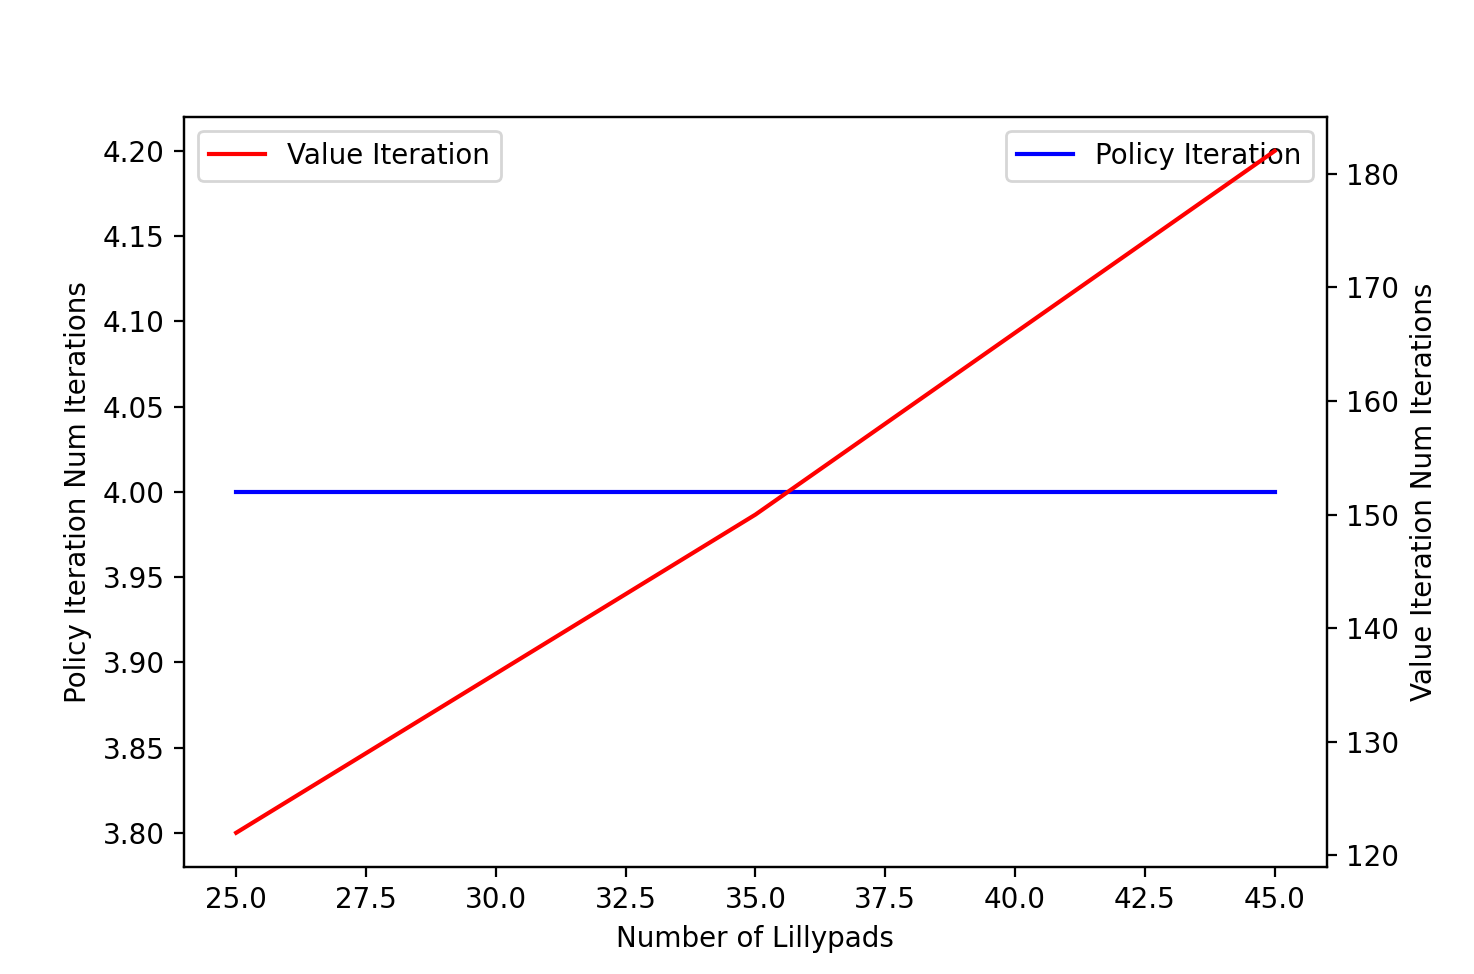
\includegraphics[width=\linewidth]{CovergenceSpeed.png}
  \caption{Iterations needed for convergence}
  \label{fig:llp3}
\end{figure}

\section{Job Hopping and Wages-Utility Maximisation}
The state will be a tuple $s_t = (s,i)$ with $s\in\{\tilde{e}, \tilde{u}\}$ and $i \in [1,2,\ldots,n]$.\\
The action space will be:
\begin{align*}
A_t(s,i) = \begin{cases} \{A\} \text{ if $s = \tilde{e}$} \\ \{A, R\} \text{ if $s=\tilde{u}$}\end{cases}
\end{align*}
The transition probabilities will be as follows:
\begin{align*}
P((s,i), A, (\tilde{e},j) &= (1-\alpha)\delta_{ij}\\
P((s,i), A, (\tilde{u},j) &= \frac{\alpha}{n}\\
P((\tilde{u},i), R, (\tilde{u},j) &= \frac{1}{n}\\
\end{align*}
With all other transition probabilities being zero. The reward function is:
\begin{align*}
R((\tilde{e},i), A, (s,j)) = \log(w_i)\\
R((\tilde{u},i), A, (\tilde{e},j) = \log(w_j)\\
R((\tilde{u},i), R, (s,j) = \log(w_0)\\
\end{align*}

This yields the following Bellman equations:
\begin{align*}
V(\tilde{e}, i) &= \log(w_i) + (1-\alpha)\gamma V(\tilde{e},i) + \frac{\alpha\gamma}{n} \sum_{j=1}^n V(\tilde{u}, j)\\
V(\tilde{u}, i) &= \max\{\log(w_i) + (1-\alpha)\gamma V(\tilde{e},i) + \frac{\gamma\alpha}{n} \sum_{j=1}^n V(\tilde{u}, j), \log(w_0)+ \frac{\gamma}{n} \sum_{j=1}^n V(\tilde{u}, j)\}\\
\end{align*}
And we can rearrange these to get:
\begin{align*}
V(\tilde{e}, i) &= \frac{\log(w_i) + \frac{\alpha\gamma}{n} \sum_{j=1}^n V(\tilde{u}, j)}{1-\gamma(1-\alpha)}\\
V(\tilde{u}, i)& =  \max\{V(\tilde{e},i), \log(w_0)+ \frac{\gamma}{n} \sum_{j=1}^n V(\tilde{u}, j)\} \\
\end{align*}
Which one step further yields:
\begin{align*}
V(\tilde{e}, i) &= \frac{\log(w_i) + \frac{\alpha\gamma}{n} \sum_{j=1}^n V(\tilde{u}, j)}{1-\gamma(1-\alpha)}\\
V(\tilde{u}, i)& =  \max\{ \frac{\log(w_i) + \frac{\alpha\gamma}{n} \sum_{j=1}^n V(\tilde{u}, j)}{1-\gamma(1-\alpha)}, \log(w_0)+ \frac{\gamma}{n} \sum_{j=1}^n V(\tilde{u}, j)\} \\
\end{align*}

We can now hence implement an algorithm that repeatedly updates $V(\tilde{u}, i)$ and then once it converges, calculate the final $V(\tilde{e}, i)$. This is implemented in worker.py. The start point for $V(\tilde{u}, i)$ is the "worst case" scenario of being unemployed for ever: $\frac{1}{1-\gamma}{\log(w_0)}$.

\section{Two Store Inventory Problem}
We adapt the problem to the given two store setup by making a few changes. First our state is now the combined state of the two stores
$$ S = \{(\alpha_1,\beta_1,\alpha_2,\beta_2) | \alpha_1+\beta_1 \leq C_1,  \alpha_2+\beta_2 \leq C_2\}  $$

We also change the action set to being the set for a given $s =(\alpha_1,\beta_1,\alpha_2,\beta_2) $:
$$A_s \{(o_1,o_2, t) \in \mathbb{N}\times \mathbb{N}\times\mathbb{Z}|-\alpha_2\leq t\leq\alpha_1,0 \leq \alpha_1 +\beta_1- t + o_1 \leq C_1, 0 \leq \alpha_2 +\beta_2+ t + o_1 \leq C_2 \}$$
where $t$ now denotes the the internal move between the stores. Note that because the internal move arrives the next morning an analogous breakdown of product shortage as in the one store cases yields 4 cases for the probability distribution using $x_1\sim Poi(\lambda_1)$.$x_2\sim Poi(\lambda_2)$.\\
Neither store runs out of inventory the next day, meaning that $x_1\leq \alpha_1 - t + \beta_1$ and $x_2\leq \alpha_2 + t + \beta_2$ and the return is the carry cost (after internal move), costs of transportation and no stock out costs. Since $x_1,x_2$ assumed to be independent we use the respective PDFs to compute the probability for this outcome.\\
Both stores run out of inventory the next day, meaning that $x_1> \alpha_1 - t + \beta_1$ and $x_2> \alpha_2 + t + \beta_2$ and the return is the carry cost (after internal move), costs of transportation and both stock out costs. Since $x_1,x_2$ assumed to be independent we use the respective CDFs to compute the probability for this outcome.\\
One of the store, say store 1, runs out of inventory the next day, meaning that $x_1> \alpha_1 - t + \beta_1$ and $x_2\leq \alpha_2 + t + \beta_2$ and the return is the carry cost (after internal move), costs of transportation and stock out costs for store. Since $x_1,x_2$ assumed to be independent we use the CDF for store 1  to compute the probability for this outcome. \\
Analogous reasoning can be used for when store 2 runs out of inventory. \\

The result is coded up in the twoStore\_inventory\_mdp\_cap.py script and yields intuitively reasonable results including ordering from the store when both stores are low on inventory and transferring internally when one store has a lot of inventory and more coming in while the other has none coming in on the previous order.

\end{document}
